\documentclass{ximera}[font=12pt]

\title{Subtracting Integers: KCC Rule}   % Use xmlatex all -s to compile when SERVE refuses to work.
\author{Kelly Stady}
\license{CC: 0}         % replace with an appropriate license, or set it in xmPreamble

\begin{document}

\begin{abstract}

\end{abstract}

\maketitle
\label{xim:SubtractIntKCCActivity}

\section*{Keep-Change-Change Rule}

The Keep-Change-Change rule is a clever way to remember how to rewrite any subtraction problem as an addition problem.

\begin{procedure}[\textbf{Keep-Change-Change Rule}]

Any subtraction problem can be rewritten as an equivalent addition problem using the steps below.

\begin{enumerate}
\item \textbf{Keep} the sign of the first number.

\item \textbf{Change} the operation of subtraction to addition.

\item \textbf{Change} the sign of the second number.

\end{enumerate}

\textcolor{accessibleOrange}{\textbf{Remember:}}  \ Subtracting a number is the same as adding the opposite of that number.
\end{procedure}



\begin{example}  

Use the Keep-Change-Change rule to find the difference $-60 - (-10).$

\begin{explanation}


The diagram below demonstrates how to rewrite the subtraction problem $-60 - (-10)$ as an addition problem.
Starting from the left, we \textbf{keep} the sign of the first number, \textbf{change} the operation of addition to subtraction, then
\textbf{change} the sign of the last number.  Lastly, we add to find the result.

\begin{center}
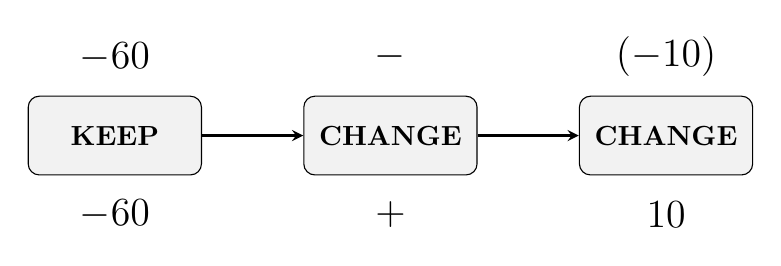
\begin{tikzpicture}[node distance=3.5cm]
    % Style definition for the Action Boxes
    \tikzset{box/.style={rectangle, rounded corners, minimum width=2.2cm, minimum height=1cm,
             text centered, draw=black, fill=gray!10, font=\bfseries}}
    \tikzstyle{arrow} = [thick,->,>=stealth]

    % Main Action Boxes
    \node (step1) [box] {KEEP};
    \node (step2) [box, right of=step1] {CHANGE};
    \node (step3) [box, right of=step2] {CHANGE};

    % Original Numbers (ABOVE) - Added \Large
    \node [above of=step1, yshift=-2.5cm] {\Large $-60$};
    \node [above of=step2, yshift=-2.5cm] {\Large $-$};
    \node [above of=step3, yshift=-2.5cm] {\Large $(-10)$};

    % Transformed Numbers (BELOW) - Added \Large
    \node (new1) [below of=step1, yshift=2.5cm] {\Large $-60$};
    \node (new2) [below of=step2, yshift=2.5cm] {\Large $+$};
    \node (new3) [below of=step3, yshift=2.5cm] {\Large $10$};

    % Arrows connecting the boxes
    \draw [arrow] (step1) -- (step2);
    \draw [arrow] (step2) -- (step3);

    % Final equation result
    %\node [below of=new2, xshift = -2cm, yshift=2.5cm] {\large $-60 - (-10) = -60 + 10$};
\end{tikzpicture}
\xmalt{A horizontal flowchart showing the Keep-Change-Change rule for the expression negative sixty 
minus negative ten.  Three boxes are arranged from left to right. The first box is labeled KEEP with 
the number negative sixty above and below it.  An arrow points to the second box, labeled CHANGE, which 
shows a subtraction sign above it changing to an addition sign below it.  A second arrow points to the third box, 
labeled CHANGE, which shows negative ten above it changing to positive ten below it. }
\end{center}


\begin{eqnarray*}
-60 - (-10) &=& -60 + 10  \\
            &=& \answer{-50}  
\end{eqnarray*}

\end{explanation}

\end{example}



\begin{example}  

Use the Keep-Change-Change rule to find the difference $40-55.$
    
\begin{explanation}


The diagram below demonstrates how to rewrite the subtraction problem $40 - 55$ as an addition problem.
Starting from the left, we \textbf{keep} the sign of the first number, \textbf{change} the operation of addition to subtraction, then
\textbf{change} the sign of the last number.  Lastly, we add to find the result.


\begin{center}
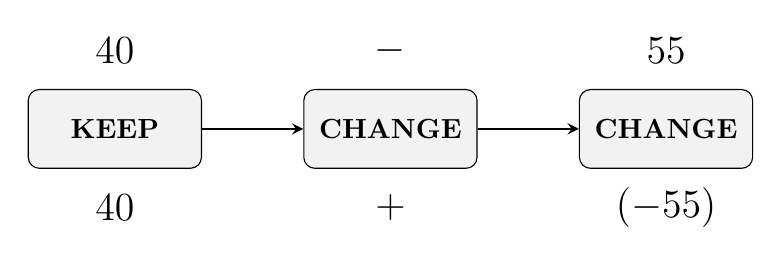
\begin{tikzpicture}[node distance=3.5cm]
    % Style definition for the Action Boxes
    \tikzset{box/.style={rectangle, rounded corners, minimum width=2.2cm, minimum height=1cm,
             text centered, draw=black, fill=gray!10, font=\bfseries}}
    \tikzstyle{arrow} = [thick,->,>=stealth]

    % Main Action Boxes
    \node (step1) [box] {KEEP};
    \node (step2) [box, right of=step1] {CHANGE};
    \node (step3) [box, right of=step2] {CHANGE};

    % Original Numbers (ABOVE) - Added \Large
    \node [above of=step1, yshift=-2.5cm] {\Large $40$};
    \node [above of=step2, yshift=-2.5cm] {\Large $-$};
    \node [above of=step3, yshift=-2.5cm] {\Large $55$};

    % Transformed Numbers (BELOW) - Added \Large
    \node (new1) [below of=step1, yshift=2.5cm] {\Large $40$};
    \node (new2) [below of=step2, yshift=2.5cm] {\Large $+$};
    \node (new3) [below of=step3, yshift=2.5cm] {\Large $(-55)$};

    % Arrows connecting the boxes
    \draw [arrow] (step1) -- (step2);
    \draw [arrow] (step2) -- (step3);

\end{tikzpicture}
\xmalt{A horizontal flowchart showing the Keep-Change-Change rule for the expression forty minus fifty five.  
Three boxes are arranged from left to right.  The first box is labeled KEEP with 
the number forty above and below it.  An arrow points to the second box, labeled CHANGE, which 
shows a subtraction sign above it changing to an addition sign below it.  A second arrow points to the third box, 
labeled CHANGE, which shows negative fifty five above it changing to positive fifty five below it.}
\end{center}

%Full left-align to make eqnarray start on left
\begin{eqnarray*}
40 - 55 &=& 40 + (-55) \\
     &=& \answer{-15} 
\end{eqnarray*}

\end{explanation}
\end{example}
               

\begin{problem} 
    Use the \textbf{Keep-Change-Change} rule to rewrite the subtraction problem as an equivalent addition problem. Then find the answer.

    \[ -8 - (-10) \]

\begin{multipleChoice}
    \choice[correct]{$-8 + 10 $}
    \choice{$-8 - 10 $}
    \choice{$8 + 10$}
    \choice{$8 - 10$}
\end{multipleChoice}


\textcolor{accessibleOrange}{\textbf{Answer}} = $\answer{2}$ 

\end{problem}





\begin{problem}
Use the \textbf{Keep-Change-Change} rule to rewrite the subtraction problem as an equivalent addition problem. Then find the answer.

    \[ 200 - (-300) \]

\begin{multipleChoice}
    \choice[correct]{$200 + 300$}
    \choice{$200 - 300$}
    \choice{$-200 + 300$}
    \choice{$-200 - 300$}
\end{multipleChoice}

\textcolor{accessibleOrange}{\textbf{Answer}} = $\answer{500}$
\end{problem}

\begin{problem}
Use the \textbf{Keep-Change-Change} rule to rewrite the subtraction problem as an equivalent addition problem. Then find the answer.
\[ 6 - 7 \]

\begin{multipleChoice}
    \choice[correct]{$6 + (-7)$}
    \choice{$6 + 7$}
    \choice{$-6 + (-7)$}
    \choice{$-6 + 7$}
\end{multipleChoice}

\textcolor{accessibleOrange}{\textbf{Answer}} = $\answer{-1}$
\end{problem}


\begin{problem}
Use the \textbf{Keep-Change-Change} rule to rewrite the subtraction problem as an equivalent addition problem. Then find the answer.

    \[ -90 - (-20) \]

\begin{multipleChoice}
    \choice[correct]{$-90 + 20$}
    \choice{$-90 - 20$}
    \choice{$90 + 20$}
    \choice{$90 - 20$}
\end{multipleChoice}

\textcolor{accessibleOrange}{\textbf{Answer}} = $\answer{-70}$

\end{problem}



\begin{problem}
Is the operation of subtraction commutative?  In other words, can we change the order of the numbers in a subtraction problem and still get the same result?

\begin{multipleChoice}
    \choice{Yes}
    \choice[correct]{No}
\end{multipleChoice}

\begin{feedback}
Subtraction is \textbf{not} commutative because swapping the order of the numbers changes the sign of the final answer.  For example, $10 - 4 = 6$ but
if we change the order of the numbers, we get a completely different result.

\begin{align*}
  4 - 10 &= 4 + (-10) \\
         &= -6 \\
\end{align*} 

Since $6 \neq -6,$ you can see that changing the order changes the result!
\end{feedback}
\end{problem}

\begin{remark}
    The rules for adding and subtracting integers apply to all real numbers. 
    The integers, along with the fractions and decimals between them make up the set of \textbf{real numbers}.  This means we 
    can apply these rules when we add and subtract fractions and decimals. 
\end{remark}

\end{document}